\documentclass[12pt,pdflatex]{elsarticle}

%%%%%%%%%%%%%%%%%%%%%%%%%%%%%%%%%%%%%%%%%%%%%%%%%%
%%%%%%%%%%%%%%%%%%%% PREAMBLE %%%%%%%%%%%%%%%%%%%%
%%%%%%%%%%%%%%%%%%%%%%%%%%%%%%%%%%%%%%%%%%%%%%%%%%


% -------------------- defaults -------------------- %
% load lots o' packages

% references
\usepackage{natbib}

% Fonts
\usepackage[default,oldstyle,scale=0.95]{opensans}
\usepackage[T1]{fontenc}
% \usepackage{ae}
% to colorize links in document. See color specification below
\usepackage[pdftex,hyperref,x11names]{xcolor}
% load the hyper-references package and set document info
\usepackage[pdftex]{hyperref}

% Generate some fake text
\usepackage{blindtext}

% layout control
\usepackage{geometry}
\geometry{verbose,tmargin=1.25in,bmargin=1.25in,lmargin=1.1in,rmargin=1.1in}
\usepackage{parallel}
\usepackage{parcolumns}
\usepackage{fancyhdr}

% math typesetting
\usepackage{array}
\usepackage{amsmath}
\usepackage{amssymb}
\usepackage{amsfonts}
\usepackage{relsize}
\usepackage{mathtools}
\usepackage{bm}
\usepackage[%
decimalsymbol=.,
digitsep=fullstop
]{siunitx}

% restricts float objects to be inserted before end of section
% creates float barriers
\usepackage[section]{placeins}

% tables
\usepackage{tabularx}
\usepackage{booktabs}
\usepackage{multicol}
\usepackage{multirow}
\usepackage{longtable}

% to adapt caption style
\usepackage[font={small},labelfont=bf]{caption}

% footnotes at bottom
\usepackage[bottom]{footmisc}

% to change enumeration symbols begin{enumerate}[(a)]
\usepackage{enumerate}

% to make enumerations and itemizations within paragraphs or
% lines. f.i. begin{inparaenum} for (a) is (b) and (c)
\usepackage{paralist}

% graphics stuff
\usepackage{subfigure}
\usepackage{graphicx}
\usepackage[space]{grffile} % allows us to specify directories that have spaces
\usepackage{placeins} % prevents floats from moving past a \FloatBarrier
\usepackage{tikz}
\usetikzlibrary{arrows, positioning, shapes.geometric,calc}
\usepackage{rotating}

% Spacing
\usepackage[doublespacing]{setspace}

% Add some colors
\definecolor{red1}{RGB}{253,219,199}
\definecolor{red2}{RGB}{244,165,130}
\definecolor{red3}{RGB}{178,24,43}

\definecolor{green1}{RGB}{229,245,224}
\definecolor{green2}{RGB}{161,217,155}
\definecolor{green3}{RGB}{49,163,84}

\definecolor{blue0}{RGB}{255,247,251}
\definecolor{blue1}{RGB}{222,235,247}
\definecolor{blue2}{RGB}{158,202,225}
\definecolor{blue3}{RGB}{49,130,189}
\definecolor{blue4}{RGB}{4,90,141}

\definecolor{purple1}{RGB}{191,211,230}
\definecolor{purple2}{RGB}{140,150,198}
\definecolor{purple3}{RGB}{140,107,177}

\definecolor{brown1}{RGB}{246,232,195}
\definecolor{brown2}{RGB}{223,194,125}
\definecolor{brown3}{RGB}{191,129,45}

\definecolor{cyan1}{RGB}{224,255,255}
\definecolor{cyan2}{RGB}{0,200,200}
\definecolor{cyan3}{RGB}{0,139,139}

% -------------------------------------------------- %


% -------------------- page template -------------------- %

\setlength{\headheight}{15pt}
\setlength{\headsep}{20pt}
\pagestyle{fancyplain}

\fancyhf{}

\lhead{\fancyplain{}{}}
\chead{\fancyplain{}{Networks \& State Preferences}}
\rhead{\fancyplain{}{}}
\rfoot{\fancyplain{}{\thepage}}

% ----------------------------------------------- %


% -------------------- customizations -------------------- %

% easy commands for number propers
\newcommand{\bl}[1]{{\mathbf #1}}
\newcommand{\first}{$1^{\text{st}}$}
\newcommand{\second}{$2^{\text{nd}}$}
\newcommand{\third}{$3^{\text{rd}}$}
\newcommand{\nth}[1]{${#1}^{\text{th}}$}

% easy command for boldface math symbols
\newcommand{\mbs}[1]{\boldsymbol{#1}}

% command for R package font
\newcommand{\pkg}[1]{{\fontseries{b}\selectfont #1}}

% approx iid
\newcommand\simiid{\stackrel{\mathclap{\normalfont\mbox{\tiny{iid}}}}{\sim}}

% -------------------------------------------------------- %

%%%%%%%%%%%%%%%%%%%%%%%%%%%%%%%%%%%%%%%%%%%%%%%%%%
%%%%%%%%%%%%%%%%%%%% DOCUMENT %%%%%%%%%%%%%%%%%%%%
%%%%%%%%%%%%%%%%%%%%%%%%%%%%%%%%%%%%%%%%%%%%%%%%%%

% remove silly elsevier preprint note
\makeatletter
\def\ps@pprintTitle{%
 \let\@oddhead\@empty
 \let\@evenhead\@empty
 \def\@oddfoot{}%
 \let\@evenfoot\@oddfoot}

\def\input@path{
	{C:/Users/Owner/Dropbox/Research/Carbon/Graphics/},
	{C:/Users/herme/Dropbox/Research/Carbon/Graphics/},
	{C:/Users/S7M/Dropbox/Research/Carbon/Graphics/},
	{/Users/janus829/Dropbox/Research/Carbon/Graphics/},
	{/Users/s7m/Dropbox/Research/Carbon/Graphics/},
	{/Volumes/Samsung_X5/Dropbox/Research/Carbon/Graphics/},
	{/Users/maxgallop/Dropbox/Carbon/Graphics/}
	}

\graphicspath{
	{C:/Users/Owner/Dropbox/Research/Carbon/Graphics/},
	{C:/Users/herme/Dropbox/Research/Carbon/Graphics/},
	{C:/Users/S7M/Dropbox/Research/Carbon/Graphics/},
	{/Users/janus829/Dropbox/Research/Carbon/Graphics/},
	{/Users/s7m/Dropbox/Research/Carbon/Graphics/},
	{/Volumes/Samsung_X5/Dropbox/Research/Carbon/Graphics/},
	{/Users/maxgallop/Dropbox/Carbon/Graphics/}
	}

\makeatother

\usepackage{etoolbox}
\makeatletter
    \patchcmd{\@author}{\global\let\@fnmark\@empty}{\global\let\@fnmark\@empty\global\let\@corref\@empty}{}{\@latex@error{Failed to patch \string\@author for \string\@corref reset}}
\makeatother

\journal{}

\begin{document}

% saying hello ----------------------------------------------- %
\thispagestyle{empty}
\begin{frontmatter}

\title{A Network Approach to Measuring State Preferences}
% \title{A Network Approach to Measuring State Preferences \tnoteref{t1}}
% \tnotetext[label1]{Author order is alphabetical.}

% \tnotetext[t1]{Thanks to people.}

% \author[strath]{Max Gallop}
% \ead{max.gallop@strath.ac.uk}
% \author[msu]{Shahryar Minhas\corref{cor1}}
% \ead{minhassh@msu.edu}
% %
% \cortext[cor1]{Corresponding author}
% %
% \address[strath]{Departments of Political Science, University of Strathclyde}
% \address[msu]{Department of Political Science, Michigan State University}

\begin{abstract}
\singlespacing{State preferences play an important role in international politics. Unfortunately, actually observing and measuring these preferences is impossible. In general, scholars have tried to infer preferences using either UN voting or alliance behavior. The two most notable measures of state preferences that have flowed from this research area are ideal points (Bailey et al., 2017) and S-scores (Signorino \& Ritter, 1999). The basis of both these models is a spatial weighting scheme that has proven useful but discounts higher-order effects that might be present in relational data structures such as UN voting and alliances. We begin by arguing that both alliances and UN voting are simply examples of the multiple layers upon which states interact with one another. To estimate a measure of state preferences, we utilize a tensor decomposition model that provides a reduced-rank approximation of the main patterns across the layers. Our new measure of preferences plausibly describes important state relations, and yields important insights on the relationship between preferences, democracy, and international conflict. Additionally, we show that a model of conflict using this measure of state preferences decisively outperforms models using extant measures when it comes to predicting conflict in an out-of-sample context.}
\end{abstract}

% journal abstract
% State preferences play an important, yet under discussed role in international politics. This is in large part because actually observing these preferences is impossible. Scholars have tried to infer preferences using UN voting or alliance behavior. Two notable measures of state preferences that have flowed from this research are ideal points and S Scores. These models use a spatial weighting scheme that discounts higher-order effects. We argue that UN voting and alliances are examples of the multiple layers upon which states interact with one another. To estimate state preferences from this multilayer structure, we introduce a latent factor model that provides a reduced-rank approximation of the main patterns across the layers. Our new measure of preferences plausibly describes important state relations. A model of conflict that uses this measure of state preferences decisively outperforms models using extant measures in predicting conflict in an out of sample context.

\end{frontmatter}
% ----------------------------------------------- %

\newpage\setcounter{page}{1}

\section*{Why we care about preferences}

% If we want to understand how two states interact in international politics, we need to know how similar their foreign policy preferences are.

Understanding state interactions in the realm of international politics necessitates some knowledge of states' foreign policy preferences vis-\`{a}-vis each other.  We can consider each state to have a preferred policy outcome on each possible issue that might arise in international relations. We can conceive of these preferred outcomes as an ideal point in multidimensional space. Given the fact that many issues in international politics are related, we can represent these preferences in far fewer dimensions than there are issues in international politics. These preferences will also change over time. When states have similar preferences on an issue, they will be more likely to collaborate to achieve their joint preference on that issue, and more generally states with similar foreign policy preferences will be cooperative in a larger proportion of their interactions. States with similar preferences are also unlikely to be involved in violent disputes with each other because the policy benefits of these disputes are unlikely to surpass the cost of fighting. Conversely, when states have highly dissimilar foreign policy preferences, cooperation will be difficult and violence will be more common. Unfortunately, while we have abundant data to measure the strength of states' economies, the volume of trade between states, or even their military power, it is much more difficult to measure states' preferences, because as with many social and political constructs they cannot be observed directly.

Effectively measuring state preferences would yield scholars a number of benefits. A number of formal theories of international relations require measures of preferences to be tested: the expected utility theory proffered by \citep{buenodemesquita:1983} has similarity of preferences as an important input. Further attempts to expand studies of crisis bargaining to include mediation \citep{kydd:2003}, coalitional dynamics \citep{wolford:2014}, or the possibility of additional disputants \citep{gallop:2017} require a measure of state preferences in order to predict whether war will be the result of bargaining failure. Preferences have been used in empirical studies predicting bilateral trade, foreign aid, stability of international institutions and the incidence of conflict \citep{derouen:heo:2004, stone:2004, gartzke:2007, kastner:2007, braumoeller:2008}. 

A substantive theoretical reason for why we need a good measure of preferences is to correctly understand the democratic peace. It is difficult to entangle whether democracies avoid war with other democracies because of the intrinsic nature of democracy, or simply because they appear to share similar ends. \citet{farber:gowa:1995} argue that democracies were only peaceful during the Cold War period because they had similar preferences and alliance structures. Similarly, \citet{gartzke:1998} argues that dissimilar preferences are a necessary condition for conflict. \citet{oneal:russett:1999e} respond by arguing that democracy has both a direct inhibiting effect on conflict, and an indirect one through influencing state preferences.\footnote{\citet{gartzke:2000} argued that even though democracies might have similar preferences, the residual of preferences from democracy explains conflict much better than the residual of democracy from preferences.} While there has been some impressive development with measures of preferences in recent years, a more accurate measure is essential to disentangle the extent to which peace is the product of shared preferences, and the extent to which institutions and norms are driving peace.

%To provide this more accurate measure we take a multilayer network based approaches to estimating state preferences. Much of the extant literature has employed spatial weighting models \citep{signorino:ritter:1999,bailey:etal:2015} on relational data such as alliance behavior and UN voting scores. We make  

Much of the extant literature has focused on estimating state preferences by utilizing spatial weighting models on either alliance behavior or United Nations (UN) voting scores. These approaches have proven to be useful but there are two reasons to desire a different approach. First, alliances are rare and voting together in the UN is very common, so, by only focusing on the direct dyadic behavior, we risk mischaracterizing important relationships. Second, we would expect a better understanding of state preferences to help us predict state behavior, but as we show in Figure \ref{fig:rocShitty} adding measures of state preferences to a traditional model of interstate disputes yields relatively scant increases in terms of predictive ability.

\begin{figure}[ht]
	\centering
	\begin{tabular}{cc}
	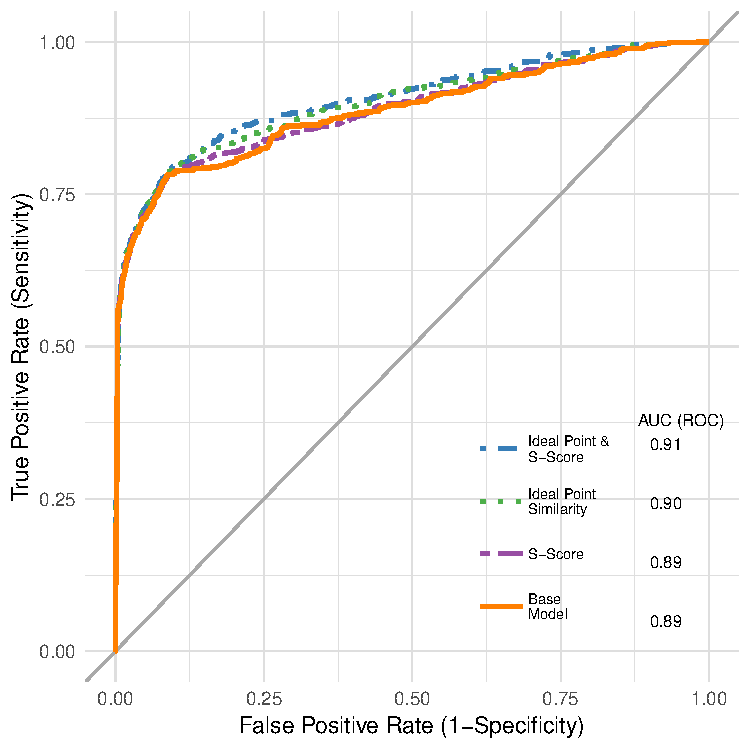
\includegraphics[width=.5\textwidth]{roc_outSample_noLatAngle.pdf} & 
	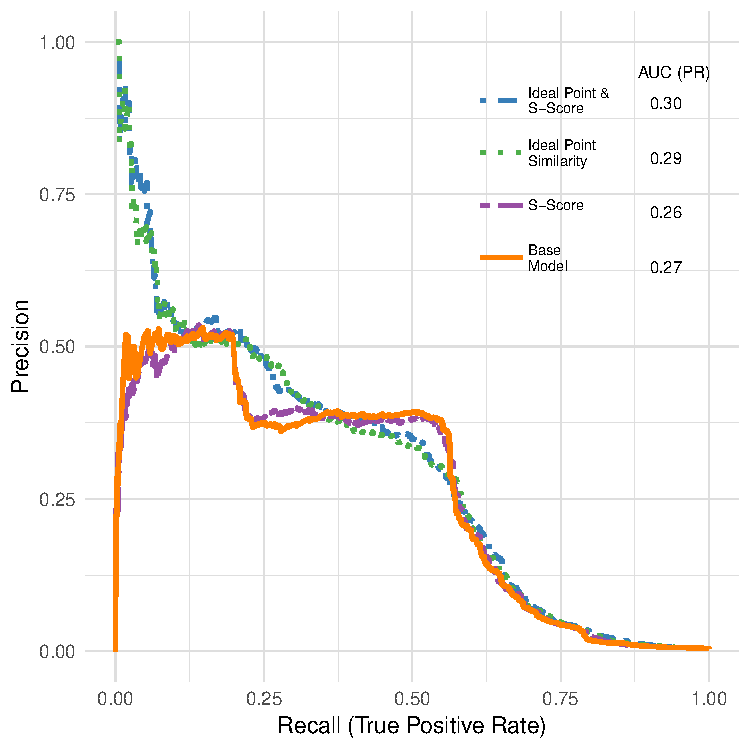
\includegraphics[width=.5\textwidth]{rocPr_outSample_noLatAngle.pdf}	
	\end{tabular}
	\caption{Assessments of out-of-sample predictive performance of Militarized Interstate Disputes using ROC curves and PR curves. AUC statistics are provided as well for both curves.}
	\label{fig:rocShitty}
\end{figure}

We can improve on these measures of preferences using the same raw material by acknowledging that both alliance membership and UN voting are layers of relationships that takes place simultaneously and in an interdependent context. Specifically, these relations between states constitute a multilayer network, in which the various layers correspond to different ways states are interacting with one another at a given time point. A bevy of research has shown that accounting for network structure necessitates an approach that can account for the indirect relations states share. As such, we make two contributions to the existing literature on state preferences. We utilize a multilinear tensor regression that enables us to measure how dependent actions of a particular dyad are across layers and time. We show that our revised approach of measuring state preferences both better characterizes relationships that have had counterintuitive results, and this measure greatly enhances our ability to predict instances of conflict.
\section*{Sources of Preference Measures: Alliance Portfolios and UN Voting}

Given that we cannot directly observe state preferences, scholars have attempted to estimate preferences using two main behavioral indicators: who states choose to ally with and how states vote at the United Nations (UN). The idea behind alliance portfolio measures is that we can infer a state's foreign policy by looking at the states they choose to align with. In the extreme case, if two states have all of the same allies, it is likely that their foreign policy goals are quite similar. Conversely, if all allies of one state are not allied to another, and vice versa, our best guess is that these states would have different aims and desires in foreign policy. \citet{buenodemesquita:lalman:2008} encapsulate the logic when they note that ``alliance commitments reflect a nation's position on major international issues''. Measures of alliance behavior do, however, suffer from the fact that these measures are largely static and sparsely occurring. Formal alliances are relatively constant over time, whereas in many cases state preferences will be more fluid, and therefore these scores will be at best a lagging indicator of preferences. Furthermore, as \citet{hage:2011} points out, the fact that links are so rare creates an artificial similarity of alliance portfolios.

We also have a relatively large corpus of behavioral information in UN Voting Records. The cost of voting in the UN is low, and so, scholars have argued that measures of affinity based on UN voting are relatively representative of the underlying distribution of preferences \citep{gartzke:1998}. This is especially fortuitous because the methodology of inferring preferences from voting in a legislature is relatively advanced. A few issues with these measures are that the potential benefit of winning UN votes is low, and so states might have incentives to vote against their preference as they are not costly signals, and the distribution of UN voting is prone to large supermajorities of the type rarely seen in ``ordinary" legislatures.

\subsection*{Current measures of preferences: S-Scores}

 The initial measure used to measure preference similarity based on alliance portfolios was Kendall's $\tau_{B}$ \citep{buenodemesquita:lalman:2008}. This measure is:
 
 \begin{equation}
	 \tau_{B} = \frac{n_{c} - n_{d}}{\sqrt{(n_{0} - n_{1})(n_{0} - n_{2})}}
 \end{equation}
 
 \noindent where $n_{c}$ is the number of pairs where both actor $i$ and $j$ have the same rank ordering (for example both the United Kingdom and the United States are more closely allied to Israel than to Iran), $n_{d}$ is the number of pairs where they have discordant rankings (the United States is more closely allied to Saudi Arabia than to Russia, Syria is more closely allied to Russia than to Saudi Arabia). The denominator attempts to adjust the total number of pairs with the number of ties: $n_{0}$ is the total number of pairs ($n(n-1)/2$), $n_{1}, n_{2}$ are measures for ties in both $i$ and $j$'s rankings respectively.
 
\citet{signorino:ritter:1999} convincingly pointed to flaws in this measure, notably its focus on rank-ordering as applied to a context where we instead care mostly about the presence or absence of an alliance. In addition, if we add additional strategically irrelevant states, we will create artificially high $\tau_{B}$ statistics. Thus, Signorino and Ritter introduce the S-score, which has since been the most widely used alliance similarity measure.\footnote{\citet{bennett:rupert:2003} also find a stronger relationship between theoretical predictions and results when using S-scores than when using $\tau_{B}$.} The equation for the S-score is:

\begin{equation}
	S(P^i, P^j, W, L) = 1 - 2w_k \frac{d(P^i, P^j, W, L)}{d^{\text{max}}(W,L)}
\end{equation}

\noindent where $d(P^i, P^j, W, L) = \sum_{k = 1}^N \frac{w_k}{\Delta^\text{max}_{k}} |p^i_k - p^j_k|$. In $d(P^i, P^j, W, L)$, $w_k$ is the $k$'th element of a weight matrix, $d^\text{max}(W,L)$ is the maximal distance on a given dimension, and $\Delta$ is a normalizing constant. For the weight matrix, generally, analysts have used S-scores calculated with a weight matrix of ones--giving each potential ally equal weight--though the other plausible choice would be to weight states by importance, for example using their share of world military capability, as calculated by \citet{singer:small:1995}. \citet{gartzke:1998} attempted to apply a similar S-score methodology to UN voting data and created the ``Affinity of Nations'' index. An important point for these scores is that they are purely dyadic. One can look at the S-score between two states, but one cannot look at a state's preferences in comparison to a larger cluster, or note the movement in a states preferences over time. In monadic analysis, these score measures are not even available, and once we are dealing with situations involving more than two states, the number of S-scores necessary to fully characterize the preferences balloons quickly (it is the number of actors choose two). 

An advantage of utilizing UN General Assembly Voting, is that it allowed the field to take advantage of methodological advances that have been made in the study of legislatures \citep{poole:rosenthal:1985}. \citet{bailey:etal:2015} do so by using an Item Response Theory model on UNGA voting. This model seeks to place states on a unidimensional latent preference space using their voting behavior. The assumption of this model is that states' votes on a resolution are a function of states' ideal points, characteristics of the vote, and random error. In particular, for each bill $v$, a state's vote will be based on the latent variable $Z_{itv}$:

\begin{equation}
	Z_{itv} = \beta_{iv}\theta_{it} + \epsilon_{iv}
\end{equation}

\noindent such that the state will vote yes if $Z_{itv} < \gamma_{1v}$, no if $Z_{itv} > \gamma_{2v}$ and otherwise abstain. Here, $\theta_{it}$ is state $i$'s ideal point at time $t$, and $\beta_{iv}$ is the discrimination parameter of a particular bill $v$. When $\beta_{v}$ is positive, states with high ideal points will be more likely to vote no. When it is negative, they will be more likely to vote yes.

The authors specifically fix the parameters $\gamma_{1v}$ and $\gamma_{2v}$ such that the same bill will have the same value in different years, and they standardize and normalize $\theta$. They also use $\theta_{it-1}$ as a prior on $\theta{it}$. With these constraints, they solve for the ideal points using a Metropolis Hastings Markov Chain Monte Carlo (MCMC).

Both methods relying on UN data, and those relying on alliances have difficulties distinguishing within '0's and '1's. For example, if we know two states are allies, we have reason to believe they have similar preferences, but if we know they are not allies, it is not clear whether they are enemies or they are indifferent -- the United States is ``not-allies" with both Bhutan and North Korea for example. As of 2012, using the Correlates of War projects alliance data, only about 1/8th of all dyads were between countries with any sort of alliance. Similarly, with UN voting, so many UN votes contain super-majorities and states vote together a huge proportion of the time. If we only look at yes and no votes in the UN general assembly, the median pair of states has voted together about 96\% of the time. If we include abstentions,  they have voted together 86\% of the time. So when two states vote together it is hard to distinguish between states voting together because of similar preferences, or just preferences that are not radically dissimilar. Both S-scores and Item Response theory succeed in adding granularity and nuance to these rough measures, but they are both limited by focusing only on a relationship between two states. 

We can see the potential issues of focusing only on direct relations when we view how these two measures of preference treat relations over the Korean peninsula. If we take China, North Korea, South Korea, and the United States, we would expect the United States and South Korea to have preferences that are similar to each other and dissimilar from China and North Korea (and vice versa). Yet, if we look at extant measures of preferences (as of 2012), as depicted in Figure \ref{korean:prefs}, they do not seem to effectively characterize this relationship. S-scores based on alliance portfolios posit that China and the two Koreas are closely clustered, with the United States distant from all three, while ideal point distances put South Korea as equidistant between the United States and North Korea. Now it could be that these measures are producing a novel, counterintuitive, result, but given the failures of extant preference measures to add much to our predictive models of conflict, one might be skeptical.

\begin{figure}[ht]
	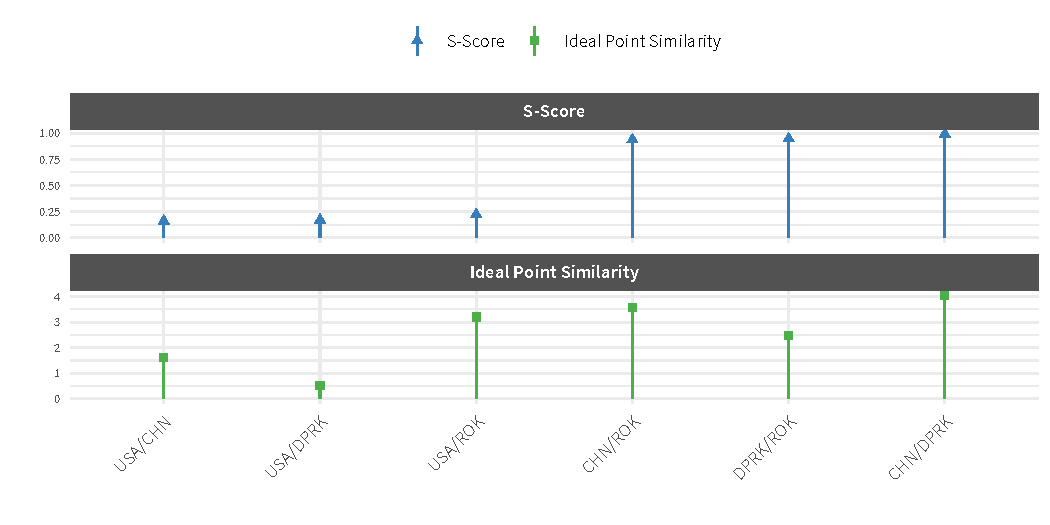
\includegraphics[width=1\textwidth]{idPtScoreViz.pdf}
	\caption{Visualization of ideal point distance and S-score relationships between China (CHN), North Korea (DPRK), South Korea (ROK), and the United States (USA) in 2012. We have rescaled each of these measures to be between 0 and 1 for comparability, where a 1 indicates that states are farther apart and a 0 that states are closer together.}
	\label{korean:prefs}
\end{figure}

The sources of these surprising results become more clear when looking at the data on which they are based. In 2012, according to the Correlates of War, North Korea only had 3 alliances -- a non-aggression pact with the South, and alliances with Russia and China. Similarly, South Korea's only alliances were that non-aggression pact, and an alliance with the United States. Given the United States' many other allies, there was much more divergence between their alliance portfolio and South Korea's, than there was between the two Koreas' portfolios \citep{gibler:sarkees:2004}. Similarly, when looking at voting patterns at the UN, South Korea voted 50\% of the time with the US, 63\% of the time with North Korea, and 70\% of the time with China.

Even using this data, we can better approximate state preferences when we treat alliances and UN voting as relational data. When it comes to alliance behavior, the fact that North Korea was allies with China and Russia, and South Korea with the United States could give us additional information, because the alliance behaviors of countries such as the United States and China are so divergent. When looking at voting patterns at the UN, the data is even more unexpected. In 2012, South Korea voted 50\% of the time with the US, 63\% of the time with North Korea, and 70\% of the time with China.

We thus argue that two changes can substantially improve our measures of state preferences. First, both alliances and UN voting contain information about state foreign policy preferences, and given the limits of this information, we should find a way to use both. Second, by using network techniques and treating this data as relational data, we can wring more information from the stone, and get both a more nuanced, and more accurate view of state affinity and state preferences.
\subsection{Synthesizing Measures of State Preference}

We propose that preferences and ideal points can be better measured by combining multiple proxies, and accounting for network interdependencies. Obviously, the idea of using multiple metrics to get a better handle on preferences is not new, in fact Signorino and Ritter suggested it in introducing S scores, which were designed to allow for aggregation of similarity on multiple dimensions (such as alliances and UN voting). What we propose, is to combine the dyadic measures of state similarity created using S-scores for alliances, and using voting models for UN data, in a manner that is both principled, and allows us to account for interdependencies. In particular, we use these two measures of state preference in a network model, in order to ascertain the state positions that best explain not only states dyadic similarity and dissimilarity on both measures, but also why states form the clusters they form. Our hope, is that by combining different measures of state preferences, and better accounting for spatial dependencies, we are able to generate a measure for preference that maintains the insights of both UN voting scores and S-scores, but which can also yield some new insights, in particular, when it comes to predicting and explaining interstate conflict.

\section{Methodology}

\subsection{AME, Why Network stuff matters}

% needs to be modified
\begin{figure}[ht]
	\centering
	\resizebox{.5\textwidth}{!}{\input{tensorViz.tex}}
	\caption{Tensor representation of longitudinal dyadic, representational measures. The green and blue colors represent different relational measures and darker shading indicates later time periods. Specifically, we show a tensor with dimensions of $4 \times 4 \times 2 \times 3$, where 4 represents the number of actors, 2 the number of relational measures, and 3 the number of time points.}
	\label{fig:tensViz}
\end{figure}

We want a model that takes a set of actions between countries, and infers each countries position in a latent preference space, such that those countries close to each other are likely to have similar preferences and therefore have similar alliances and UN voting records. We would like this methodology to be able to, in a principled way combine different sources of data, for example imputing ideal points based on both alliance behavior and behavior at the UN. Finally, and importantly, this method should be able to account for interdependencies: similarity in preferences should be transitive (if the US has similar preferences to the UK, and the UK to France, the US's preferences should be relatively close to France's) and should allow for clusters of states with similar preferences.

The Additive and Multiplicative Effects model (AME) model is a relatively new technique that is a generalization of the Generalized Bilinear Mixed-Effects model from \citet{hoff:2005}. The model is an extension of the Social Relations Model: 

\begin{equation}
	f(Y_{i,j}) =  \beta^{'}\mathbf{x_{i,j}} + \alpha_{i} + b_{j} + \epsilon_{i,j}
\end{equation}

where $f(.)$ is a general link function corresponding to the distribution of Y, $\beta^{'}\mathbf{x_{i,j}}$ is the standard regression term for dyadic and nodal fixed effects,  $\alpha_{i}, b_{j}$ are sender and receiver random effects, and $\epsilon_{i,j}$ is an IID error term. The AME model further decomposes the  error term as follows. If we assume the matrix representation of deviation from the linear predictors and random effects is $\mathbf{Z}$, then $\mathbf{Z} = \mathbf{M} + \mathbf{E}$ such that the matrix $\mathbf{E}$ represents noise, and $\mathbf{M}$ is systematic effects. By matrix theory, we can decompose $\mathbf{M} = \mathbf{UDV^{'}}$ such that $\mathbf{U}$ and $\mathbf{V}$ are are n x n matrices with othonormal columns, and $\mathbf{D}$ is an n x n diagonal matrix. This is called the singular value decomposition of $\mathbf{M}$. 

We then write the AME model for a given value $Y_{i,j} \in \{0,1\}$:

\begin{equation}
	\text{logit}(P(Y_{i,j} = 1| x_{i,j}) = \beta^{'}\mathbf{x_{i,j}} + \alpha_{i} + b_{j} + \mathbf{u_{i}Dv^{'}_{j}} + \epsilon_{i,j}
\end{equation}

In estimating preference models, we abstain from using fixed effects save an intercept.

An important innovation with the AME, as compared to previous network estimates is the ability to handle replicated datasets -- here we use the replicated dataset to incorporate multiple measures of similarity into a single ideal point estimation.  The AME with dyadic data treats each different slice of data as independent, save for those dependencies captured by the nodal and multiplicative random effects, as well as those controlled for by fixed effects. The final estimating equation we use is:

\begin{equation}
	\text{logit}(P(Y_{i,j_j} = 1) = \mu + \alpha_{i} + b_{j} + \mathbf{u_{i}Dv^{'}_{j}} + \epsilon_{i,j,t}
\end{equation}

What is particularly useful here is the eponymous multiplicative effect $\mathbf{u_{i}Dv^{'}_{j}}$. This effect not only helps to account for homophily and stochastic equivalence, it also places each state in a latent space. What is key to understand about this latent space is that it is non-euclidian. Rather than have states behave similar to the states which are close to them, this latent space is a two dimensional representation of a hypersphere, and thus states are apt to behave similarly to the states that are placed in the same direction on said sphere. Thus, if two states vectors (from the center of the space) are in the same direction, they are apt to send and receive both alliances and co-voting to similar targets. The way we measure this similarity in dimension is by looking at the absolute distance of the angles created by each states position and the center of the latent space. 

% \section{Our Approach: Using Event Data}
% We propose that one can get a useful proxy of state preferences is a more fluid and behavioral approach--using event data on cooperation and conflict to measure amity and enmity between states. Event data is (generally) machine coded data which uses news articles to capture the type and tenor of relationships between actors. The goal would be to take a measure of cooperative actions, and conflictual actions, and use these two counts to estimate each state's position in a two dimensional latent space in a given year. 

% The intuition behind this use of event data is that states are more likely to cooperate with states with similar preferences, and they are more likely to conflict with states that have divergent preferences. Similarly, we can also infer similarity by how states act towards common third parties. The reason we use event data is that it is more dynamic and representative of current preferences than data on alliance or international organization comembership (which becomes quite sticky and might represent states preferences at some point in the distant past), while at the same time it is more revealing than behavior at the United Nations, because these conflictual and cooperative actions are actually consequential, in contrast to non-binding UN resolutions.


% \subsection{ICEWS Event Data}
% To estimate state preferences. The ICEWS data were collected via a Defense Advanced Research Project Agency (DARPA) funded project that created a dataset of over two million machine-coded daily events occurring between relevant actors within twenty-nine countries in the the Asia-Pacific region. ICEWS utilized news articles from over 75 electronic regional and international news sources and machine coded these events, using the Penn State Event Data Project's TABARI (Text Analysis By Augmented Replacement Instructions) software program\citep{schrodt:vanbrackle:2013} and a commercially developed, java variant (JABARI). TABARI and JABARI used sparse parsing and pattern recognition techniques to machine-code daily political events based primarily on a categorical coding scheme developed by the Conflict and Mediation Event Observation (CAMEO) project\citep{gerner:schrodt:yilmaz:2009}. This ICEWS dataset is the current gold- standard for event data\citep[p.4]{dorazio:etal:2011}.

% For an example of how a conflictual event was coded in the data, consider the example:\footnote{Taken from the CAMEO code book, \citep{gerner:2009}.}

% \begin{quote}
% Israel today mounted its long-threatened invasion of South Lebanon, ploughing through the United Nations lines on the coast of south of Tyre and thrusting forward in at least to inland areas.
% \end{quote}

% In this sentence, Israel is coded as the source of the event, and South Lebanon is coded as the target. Then South Lebanon is aggregated with events involving the entire country of Lebanon. The event type coded in this story is ``occupy territory," coded as such because of the use of the verb ``mounted" and the noun ``invasion." Events of the type ``occupy territory" are then put into the category ``material conflict." 

% Similarly, this story from a major news service:

% \begin{quote}The Afghan foreign ministry announced that Kabul and Tehran have agreed to a prisoner exchange, a move seen by many analysts as yet another sign of warming relations between the two neighbors ahead of the planned withdrawal of foreign combat forces from Afghanistan in 2014.
% \end{quote}

% is coded as an action between Afghanistan and Iran, based on the nouns ``Kabul" and ``Tehran," and is of the event type ``express intent to release persons or property" based on the phrase ``agreed to a prisoner exchange." This type of event is coded as verbal cooperation.

% We aggregate this data to the yearly level, combined based on the concept of Quad Categories--a two by two that differentiates verbal and material acts, as well as conflictual and cooperative ones.
\subsection{Data Sources, Modeling choices}

We use the AME model on the two aforementioned measures of state amity to generate a combined measure of state preference similarity which accounts for network effects. We use the distance between states' ideal points (as calculated by \citet{bailey:strezhnev:voeten:2015} using UN data) and S-score for two states alliance portfolios. However, to facilitate comparison between the metrics, we first transform the S-score into a measure of distance between alliance portfolios.\footnote{D = 1 - S} We then standardize and normalize these two measures. This gives us an N by N by Y by 2 array, where the first two dimensions represent countries, the third dimension is the year, and the fourth is the particular measure of similarity. So the item at index (1,2,1,1) would be the transformed value of the S-score for countries XXX and YYY at the first year of our data (YYYY), similarly (1,2,1,2) would be the UN ideal point distance.

Another important question is the amount of temporal aggregation used. In our baseline model, we treat each year as separate and gain a unique observation of each states ideal point in each year. However, this raises a real risk of temporal inconsistency in the values. An alternative approach would be to have a rolling average for the measures of similarity over a number of years. This would allow us to infer a country's relative position not just by their behavior in a given year, but also their behavior in the past few years. The risk if we use too much temporal aggregation is that we are including data which is no longer relevant to a country's relative preferences. For instance, Turkey and Russia's relationship looks a lot more positive when we look at 2013 and 2014 then when we look at 2015. To that end, in addition to our baseline model where years are seen as independent, we also evaluate models where ... 

With this data, we run an AME model with a Gaussian link, and in particular we use the uDv term to estimate each states position in a two-dimensional latent space. We then evaluate whether their is additional utility gained from using this latent position, as compared to the component measures of similarity of alliance portfolio and UN ideal point distance.

\section{Constructing Latent Angle Measure}

\subsection{Face Plausibility}

An important question for these different measures of preferences, are whether they give results that ``make sense" for certain prominent pairs of countries. In particular we would hope that the measures both give sensible levels to relationships -- sorting states into friends and foes effectively -- but also that when these measures change, they do so in sensible ways, and in ways that correspond to changes in the world. We thus present all three measures' accounts of eight dyadic relationships over time.\footnote{For the sake of having each measure operate in the same direction, we transform the S-score such that the value shown is 1 - S. Thus for all three variables, $0$ implies perfect symmetry of preferences.} A note is that each of these measures is on a different scale, and so just because one measure has a higher value, does not necessarily mean that it posits more dissimilarity of preferences.

We first look at three close relationships where we'd expect to see similar preferences: as depicted in figure \ref{friendly:dyads} the relationships between France and Germany, the US and Israel, and North Korea and China. In all three cases our measure using Latent Angle distance has consistently low values -- nearly $0$ in the case of France and German, and China and North Korea, and low but less stable values for the US/Israel relationship. Alliance S-Scores correctly classify Franco-German and Sino-North Korean friendship, while the US/Israel relationship is characterized as being relatively neutral. The measure based on UN voting is most out of step in terms of characterizing these relationships, with notable divergence in the preferences of many of these pairs.

[remake these graphs]
\begin{figure}
\subfigure{\includegraphics[height = 6cm, width = 5cm]{DyadViz/FranceGermany}}
\subfigure{\includegraphics[height = 6cm, width = 5cm]{DyadViz/USIsrael}}
\subfigure{\includegraphics[height = 6cm, width = 5cm]{DyadViz/NoKoChina}}
\caption{Dyadic relationships between 3 pairs of countries according to the different preference measures. Latent angle distance is in black, ideal point distance based on UN voting is in blue. S-score has been rescaled such that it works in the same direction as the other measures (1-S-score, so that the best score is 0), and is in red.}
\label{friendly:dyads}
\end{figure}

In figure \ref{unfriendly:dyads} we look at the United States' relationship with three countries that are characterized by change and major events. The biggest difference between the measures is that alliance S-scores are the only measure that does not detect a marked improvement in the US/Russian relationship at the end of the Cold War. Both the UN ideal points and Latent Angle space find significant improvements followed by a drift toward enmity, whereas S-scores have a constant (though slightly improving) neutral relationship. For the US and Iraq no measure depicts more similar preferences following the US occupation, though only Latent Angle distance finds an increase in enmity in the run-up to the US's invasion. Finally, for the US and China, the S-score has a consistent neutral relationship, while both UN ideal points and Latent Angles have more both more negative relationships, and more variance, with Latent Angles finding particularly large spikes at the beginning of the Bush and Obama administrations.

\begin{figure}
\subfigure{\includegraphics[height = 6cm, width = 5cm]{DyadViz/USChina}}
\subfigure{\includegraphics[height = 6cm, width = 5cm]{DyadViz/USRussia}}
\subfigure{\includegraphics[height = 6cm, width = 5cm]{DyadViz/USIraq}}
\caption{Dyadic relationships between 3 pairs of countries according to the different preference measures. Latent angle distance is in black, ideal point distance based on UN voting is in blue. S-score has been rescaled such that it works in the same direction as the other measures (1-S-score, so that the best score is 0), and is in red.}
\label{unfriendly:dyads}
\end{figure}

One big difference between these measures is that Latent Angle distance has a more full time series than the other two measures, this is particularly relevant when looking at the preferences of certain rogue states, as we do in figure \ref{missing:dyads}. In both the case of Iran/Iraq and North Korea/South Korea there is no data for UN voting (and for Iran/Iraq missing data for S-scores). For the Korean relationship, Latent Angle distance better characterizes  the relationship as enmity, while S-scores treat the two as having very similar preferences. Whereas for Iran and Iraq's relationship S-scores give a consistent close preferences (where data exists), while Latent Angles show more instability, and notable elevation (though not as large as we would expect) during their war.


\begin{figure}
\centering
\subfigure{\includegraphics[height = 6cm, width = 5cm]{DyadViz/NoKoSoKo}}
\subfigure{\includegraphics[height = 6cm, width = 5cm]{DyadViz/IranIraq}}
\caption{Dyadic relationships between 2 pairs of countries according to the different preference measures. Latent angle distance is in black, ideal point distance based on UN voting is in blue. S-score has been rescaled such that it works in the same direction as the other measures (1-S-score, so that the best score is 0), and is in red.}
\label{missing:dyads}
\end{figure}

As can be seen from these relationships, the measure of preferences based on Latent Angle distance is in many cases as plausible or more than incumbent measures of preferences. While the measure has more temporal instability than S-scores or UN ideal points, in these 8 cases it often does better, and rarely worse than the other measures at conforming to our expectations of the relationships. Of course, this could just be a case of us picking particularly propitious cases. These 8 dyads show the plausibility of our measure of state preferences, but the real test is in the large-N analysis of conflict in the next section.


\section{Model Competition}

To evaluate different measures of state preferences, we compare them in a model of interstate disputes. Here we look at four non-nested models: a model using no measures of state preferences, one using an S-Score based on similarity in alliance portfolio (as in \ref{signorino:ritter:1999}, one using the ideal points determined by UN voting (as in \ref{bailey:strezhnev:voeten:2015}), a model using both UN ideal points and alliance S-scores, and finally, a model using our latent angle approach to combine data from UN voting and alliances. We evaluate the models on two criteria: whether state preferences have a consistent effect in the predicted direction, and how well each model does at predicting disputes on out of sample data.

\subsection{Data, Controls}

In each of these models, we look at a logistic regression of Militarized Interstate Dispute participation on measures of state preferences and a vector of control variables. These control variables are most of the standard ones used most famously in O'Neal and Russett's work on the democratic peace \citep{oneal:russett:1997}.\footnote{The exception is that our models ignore trade interdependency, as including that data drastically decreases the number of observations.} In particular, we include a binary measure of joint democracy (whether both states have Polity IV scores $geq 7$), whether the states are contiguous, and the ratio of state capabilities as measured by the Correlates of War Project's Composite Index of National Capabilities (CINC). We also account for temporal interdependence using a peace year spline, as in \ref{beck:etal:1998}. 

\subsection{In sample explanation}

As detailed in figure \ref{fig:coefP}, each measure of state preferences performs as we would expect them to. Our measure of state preference using latent angle difference is highly significant and positive: states with more dissimilar preferences will have greater difference in their latent angles, and this is highly associated with a greater risk of conflict. Similarly, both incumbent measures of preferences pass this test. The measure using UN voting ideal points is positive and clearly distinct from $0$, indicating that states with more distant ideal points, and thus more dissimilar preferences, are more likely to find themselves in conflict. Similarly, higher alliance S-scores are consistently associated with lower probabilities of conflict -- so states with more similar preferences as measured using alliance portfolios are less likely to quarrel. These results hold when the measure of preferences is used in isolation, or in tandem.

The models have one major difference in terms of the controls: in the model using latent angle distance, joint democracy is indistinguishable from $0$. This is particularly interesting because of one of the major criticisms of democratic peace theory is that, for one reason or another, democracies have similar preferences, and this is what actually causes peace among democracies.  Despite this dispute, most attempts to include preferences in the standard democratic peace regressions still found a consistent pacifying effect of democracy.
(as do those models with UN voting and S-scores presented here). With our measure of preferences, however, democracy's effect is negligible.


\begin{figure}[ht]
	\centering
	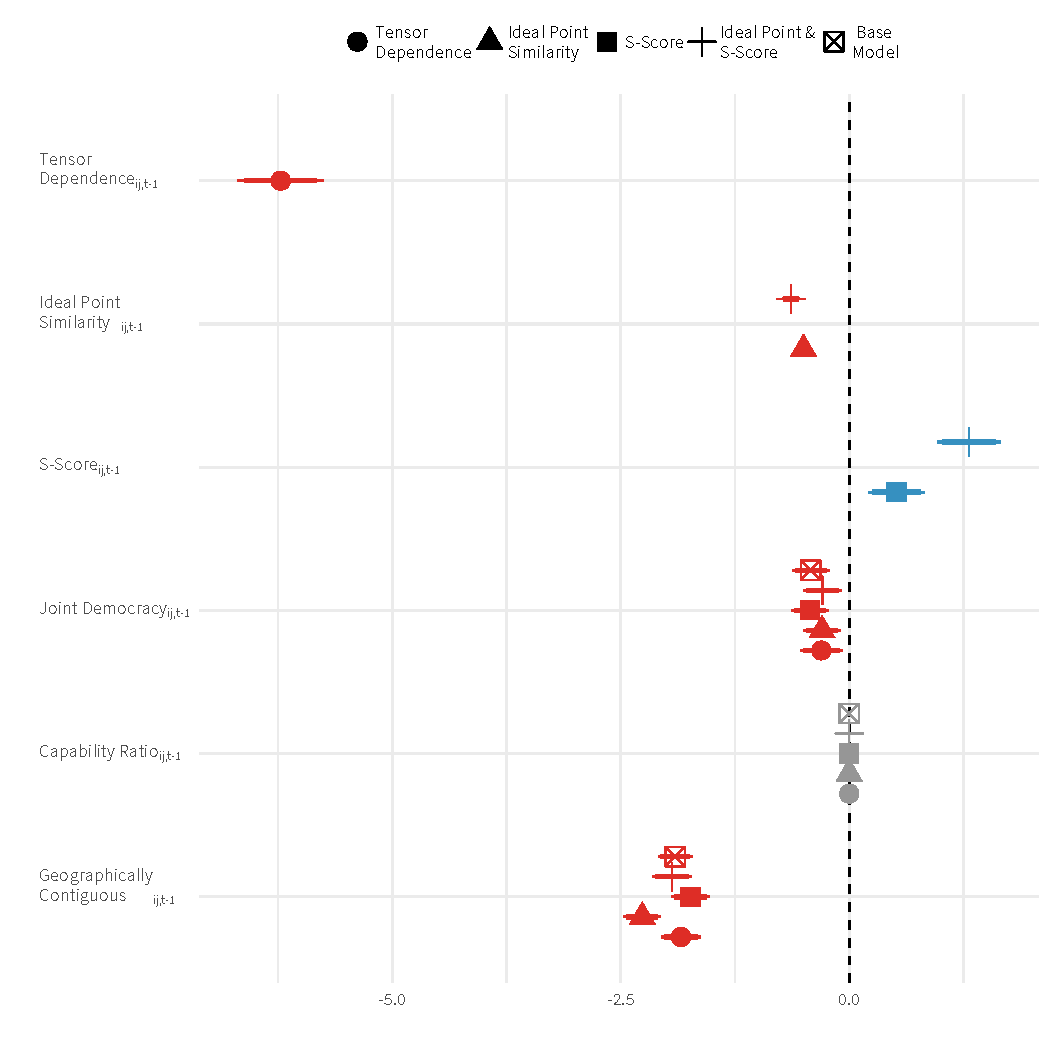
\includegraphics[width=.7\textwidth]{betaEst}
	\caption{Parameter estimates from models with different measures of state preference. Point represents average estimate, line through the point represents the 95\% confidence interval.}
	\label{fig:coefP}
\end{figure}
\FloatBarrier

\subsection{Out of sample prediction}

Given these results, we can say that all of the measures of preferences behave as we would expect. To adjudicate which measures best capture state preferences, and what we should make of the differing effect of democracy, we turn to out of sample prediction. The way we do this is by partitioning our data into 30 different folds, and for each fold we generate a predicted value for each case the other 29 folds for each model. This leaves us with a set of predicted values generated entirely out of sample. We then compare the models performance using the area under both the Receiver Operator Characteristic Curve (AUC ROC) which examines the tradeoffs between true positives and false positives, and the area under the Precision Recall Curve (AUC PR) which looks at the tradeoffs between making only correct predictions, and predicting all the disputes which occurred. In general, the AUC ROC will disproportionately reward those models that predict $0$ well, and we can interpret the AUC ROC as the likelihood a prediction is correct, the numeric value for the AUC PR has less of a clear interpretation, but models with a higher AUC PR do a better job of predicting when events actually occur.

As shown in figure \ref{fig:roc}, the model using latent angle distance decisively outperforms all the other models. While the AUC ROC is somewhat higher with the Latent Angle model, the real difference between the measures shines through in the AUC PR, where the model using this measure performs twice as well as the base model. In contrast, models using other measures of state preferences yield only minimal improvements in prediction over the base model. Thus we have real reason for confidence in both the usefulness of this measure of state preferences and renewed reason for skepticism in the effect of joint democracy once we control for state preferences. 

\begin{figure}[ht]
	\centering
	\begin{tabular}{cc}
	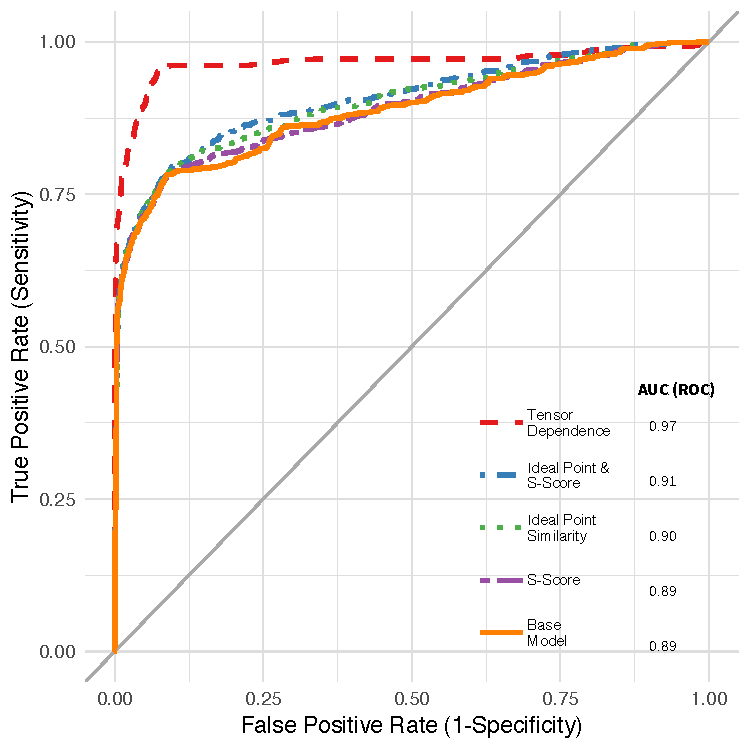
\includegraphics[width=.5\textwidth]{roc_outSample} & 
	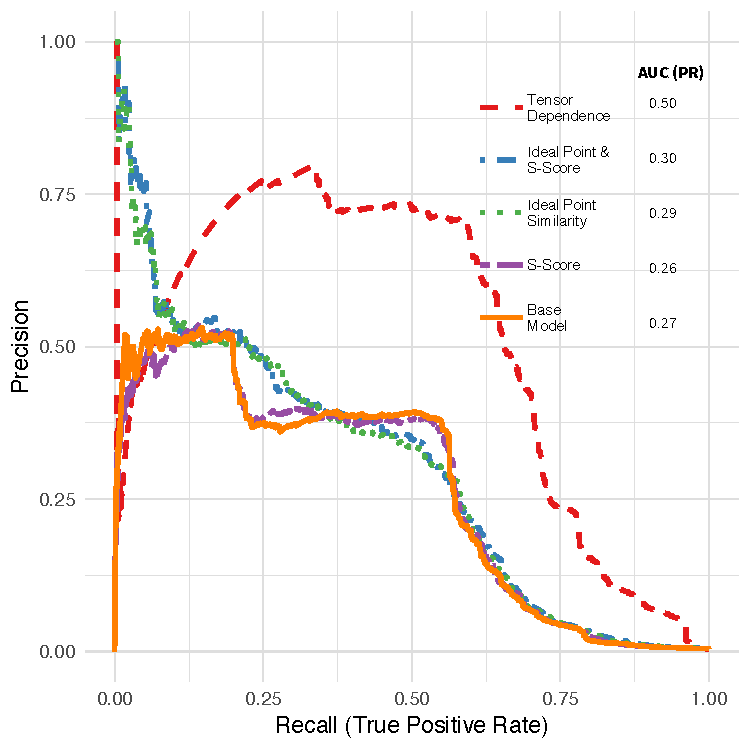
\includegraphics[width=.5\textwidth]{rocPr_outSample}	
	\end{tabular}
	\caption{Assessments of out-of-sample predictive performance using ROC curves and PR curves. AUC statistics are provided as well for both curves.}
	\label{fig:roc}
\end{figure}
\FloatBarrier


\section*{Conclusion}

We use a network methodology to create a new measure of state preference similarity using both UN Voting and alliance data. This measure of preference similarity demonstrates face plausibility comparable or superior to existing measures when it comes to capturing the dynamics of a number of notable dyadic relationships.\footnote{There is an important limitation to keep in mind with the measure that we have generated, namely that we run separate models with a fixed three year rolling temporal window to estimate this measure. In future work, exploring the value-add from employing a single model that can generate time varying measures of state preference from multiple dimensions of state relations over time would likely be of notable value. A number of works have explored measuring low-dimensional relationships between actors using dynamic latent space models (e.g., \citealp{sewell:chen:2015}), and that work will certainly prove to be informative in future work that seeks to extend these ideas to the tensor setting.}  We then attempt to use this measure of state preferences in a predictive model of interstate disputes. In doing so, we find that the measure of preferences has the expected effect (states with similar preferences are less likely to be involved in disputes). Most importantly, a model of interstate conflict that includes our measure of preference similarity decisively outperforms models that include both of the most prominent existing measures of preferences.

While this measure of state preference similarity has yielded leverage in predicting conflict, it should also be useful in answering a number of other questions. One possible use would be to look at the measure of state preferences as an outcome variable, rather than a predictor. We could here look at how preferences change in tandem with leadership change -- can we find evidence, for example, that the election of Donald Trump moved the United States' foreign policy preferences away from the major Western European states and towards Russia's? We could also see how well this measure of state preference similarity predicts more collaborative behavior -- treaty membership or trade for example.

Ours is not the first paper to use network analysis to attempt to measure a theoretically important but difficult to observe phenomenon. For example, \citet{moody:white:2003} measured social cohesion by looking at the minimum number of paths connecting each actor in a group (and applied to high school friendship networks and among American businesses. \citet{beardsley:etal:2018} generates a measure of hierarchy by looking at a network of arms transfers and first finding the clusters in each group,  then how central an actor is within a given cluster, they go on to use this measure of hierarchy in a downstream model to explain interstate conflict, and similarly \citet{cranmer:etal:2015} use a measure of multiplex modularity in the network of alliances, trade, and international organization membership to measure ``Kantian fractionalization"--the extent to which the international system is fragmented between liberal and illiberal states.

In addition to helping us to understand state preferences, this sort of technique could help in measuring phenomena like social cohesion and hierarchy, or spatial contagion. If one wanted to use network approach to measure social cohesion, one could potentially do this with a Latent Class Model as in \citet{airoldi:etal:2008}. Using some measure of social interaction, this model would give the probability that each member is in a particular clique or subgroup in society. We could then look at how many members of society have probability of membership in multiple groups above a certain threshold to see how many individuals bridge different groups, contributing to our understanding of social cohesion. In understanding how phenomenon -- violence, diseases, new technology to name a few examples -- diffuse, many scholars rely on spatial lag models, which require the scholar to specify a spatial weights matrix that indicates how likely a phenomenon is to move from one area to another. Of course, we can never know the true adjacency matrix, and so scholars use a proxy, most often some form of geographic distance. We may be able to improve the predictive performance of spatial models by inferring a weights matrix using a network approach based on how the phenomenon has diffused in the past.

In general, there are a wide variety of substantive areas in which using network models to extract measurements of how actors relate may provide new insights. We would certainly not argue that the approach we present here can easily be plugged into alternative applications.\footnote{\citet{goldenberg:etal:2010} and \citet{kim:etal:2018} provide helpful discussions of various types of network models that have emerged to study cross-sectional and multilayer networks.} In fact, despite the benefits we highlighted of our approach for measuring state preferences, there are downsides. Most notably, our choice of manually choosing the last three years of data could certainly be iterated on in future research. \citet{park:sohn:2017}, for example, present a model to actually determine when there are discrete changes in the underlying group structure of network entities. In future research, further exploring how network models can be used to address measurement problems may prove to be a fruitful area of research.

% Regardless of the model used, if you are trying to use a latent network model for measurement, and especially if you are using the measure in a downstream model, you need to be aware of and account for uncertainty. To do this, we suggest running the downstream model repeatedly with different draws from the distribution for the latent space, then combining the models using \citet{rubin:1976}'s rules to obtain an estimate of the effect of your measure that accounts for uncertainty.


\newpage

% Bib stuff
\clearpage
% \bibliography{C:/Users/Owner/whistle/master}
\bibliography{C:/Users/herme/whistle/master}
% \bibliography{C:/Users/S7M/whistle/master}
% \bibliography{/Users/s7m/whistle/master}
\bibliographystyle{elsarticle-harv}\biboptions{authoryear}

\end{document}
